\section{RESULTS AND ANALYSIS}
\subsection{Disease Prediction}
In enhancing disease prediction, the training dataset expanded from 2890 to 5175 instances, leading to a noticeable accuracy boost from 77\% to 82\%. Integrating the model with both the server and the Flutter application has been successfully achieved, marking the completion of this task.
\vspace{1cm}
\begin{figure}[ht]
  \centering
  \begin{subfigure}{0.43\textwidth}
    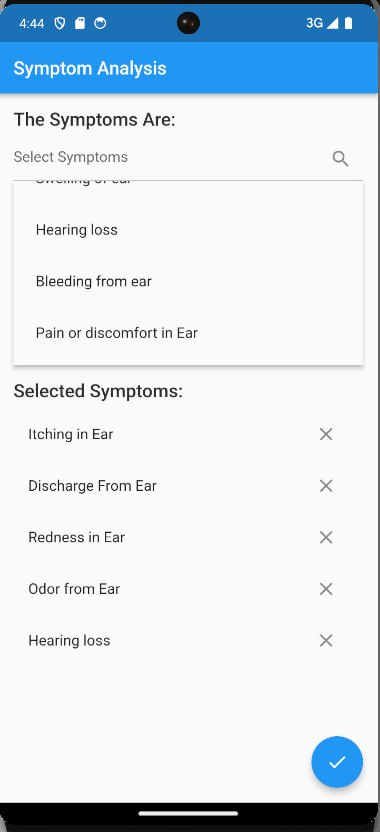
\includegraphics[width=\linewidth]{img/disease2.jpg}
    
  \end{subfigure}%
  \hfill
  \begin{subfigure}{0.44\textwidth}
    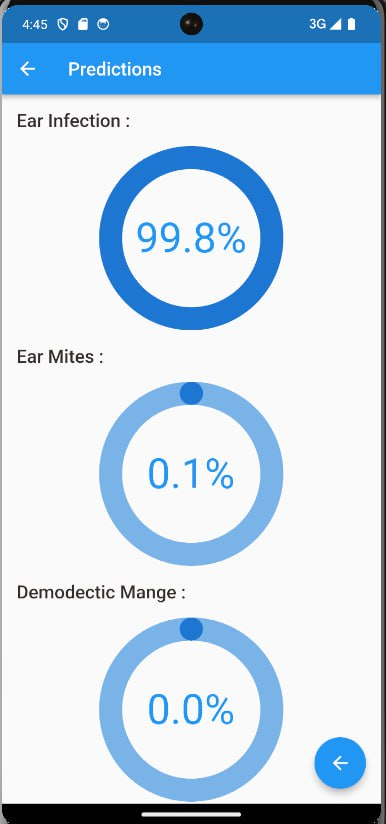
\includegraphics[width=\linewidth]{img/disease1.jpg}
  
  \end{subfigure}
  \caption{Disease Prediction}
\label{}
\end{figure}
\newpage

\subsubsection{Learning Curve}
Learning curve function from scikit-learn is used to compute the training and testing scores at different training set sizes. The mean and standard deviation of these scores are calculated and plotted on the learning curve plot. The shaded areas around the curves represent the variance in the scores. The learning curve exhibits a consistent training score of 1, indicative of potential overfitting where the model memorizes the training data excessively. Conversely, the cross-validation score demonstrates an exponential increase, reaching approximately 0.8, implying enhanced generalization as the number of training examples grows. This divergence underscores the importance of addressing overfitting concerns to achieve a more balanced and robust model.
\vspace{0.4cm}
\begin{figure}[ht]
\centering
\includegraphics[width=1\textwidth]{img/learning_curve_MLP_FINAL.pdf}
\caption{Learning Curve}
\label{fig:system-overview}
\end{figure}
The learning curve plot provides valuable insights into the performance and behavior of our model as the number of training examples increases. Notably, two distinct trends emerge, each revealing crucial aspects of our model's capabilities:

\textbf{Training Score (Red Curve):} The training score remains consistently high, hovering around 1.0, irrespective of the increasing number of training examples. This persistence at a high value indicates that our model achieves near-perfect performance on the training data. However, such sustained high performance raises concerns of overfitting, suggesting that the model may be excessively memorizing the training examples, potentially limiting its ability to generalize to unseen data.

\textbf{Cross-Validation Score (Green Curve):} In contrast, the cross-validation score exhibits a different trajectory. Starting from a relatively low value, it shows an exponential increase with the inclusion of more training examples, ultimately reaching a plateau around 0.8. This upward trend suggests that our model's generalization performance on unseen data improves significantly as it is exposed to more diverse examples during training. The observed rise in cross-validation score underscores the importance of sufficient training data in enhancing the model's ability to generalize effectively beyond the training set.
\subsubsection{Training Loss}
 Training Loss will generate a plot that shows how the training loss decreases over epochs. It can helped us assess whether the model is converging and whether we need to adjust hyperparameters such as learning rate, batch size, or the number of hidden units to improve convergence. Observing the training loss graph, it is evident that the loss rapidly decreased from 4 in the first epoch to nearly 0 over the subsequent epochs up to 50, indicating effective model convergence. However, the loss curve plateaued and remained constant beyond the 125th epoch.
\vspace{1cm}
\begin{figure}[H]
\centering
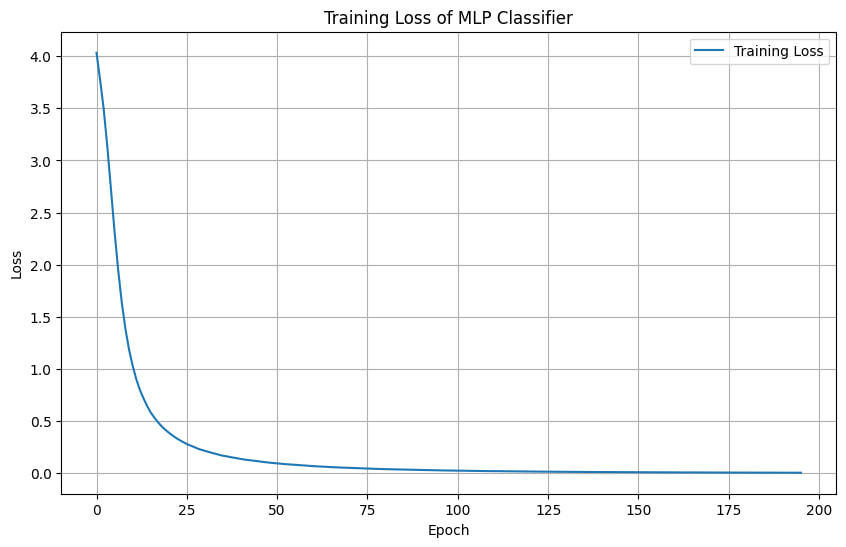
\includegraphics[width=0.7\linewidth]{img/Training Loss.jpg}
    \caption{ Training Loss}
    \label{fig:Traingin loss}
\end{figure}
\newpage

\subsubsection{Validation}
\textbf{Hidden Units}\\
The validation curve depicted in the figure below illustrates the performance of the algorithm across varying numbers of hidden units. Initially, the algorithm was trained using 50 hidden units, resulting in an accuracy of 77\%. Subsequently, the hyper parameter was systematically adjusted, culminating in the highest observed accuracy of 82\% when employing 225 hidden units.
\vspace{0.7cm}
\begin{figure}[H]
\centering
\includegraphics[width=1\linewidth]{img/validation_curve.pdf}
\caption{Validation Curve hidden Units}
\label{fig:system-overview}
\end{figure}
\newpage
\textbf{Random State}\\
The validation curve, depicting the fluctuation in accuracy as the random state parameter varies within the range of 30 to 50, is presented below. Initial observations reveal an accuracy of approximately 70\% at random state 30, followed by a subsequent rise and fall in accuracy across the range. Notably, the apex accuracy of 82\% is observed at random state 42. This trend highlights the influence of the random state parameter on model performance and underscores the importance of selecting an optimal value to maximize predictive accuracy.
\vspace{0.7cm}
\begin{figure}[H]
\centering
\includegraphics[width=1\linewidth]{img/Random State}
\caption{Validation Curve Random State}
\label{fig:system-overview}
\end{figure}
\newpage
\subsection{Breed Detection}
The breed detection model has undergone comprehensive training and refinement, enabling it to proficiently distinguish between dog images and other entities. Through batch training with expanded datasets from 16,000 to 20,000 images spanning 120 dog breeds, the accuracy surged significantly from 80.34\% to an impressive 92.22\%. This remarkable improvement attests to the model's enhanced capability and accuracy in breed identification. 

\vspace{1cm}
\begin{figure}[ht]
  \centering
  \begin{subfigure}{0.45\textwidth}
    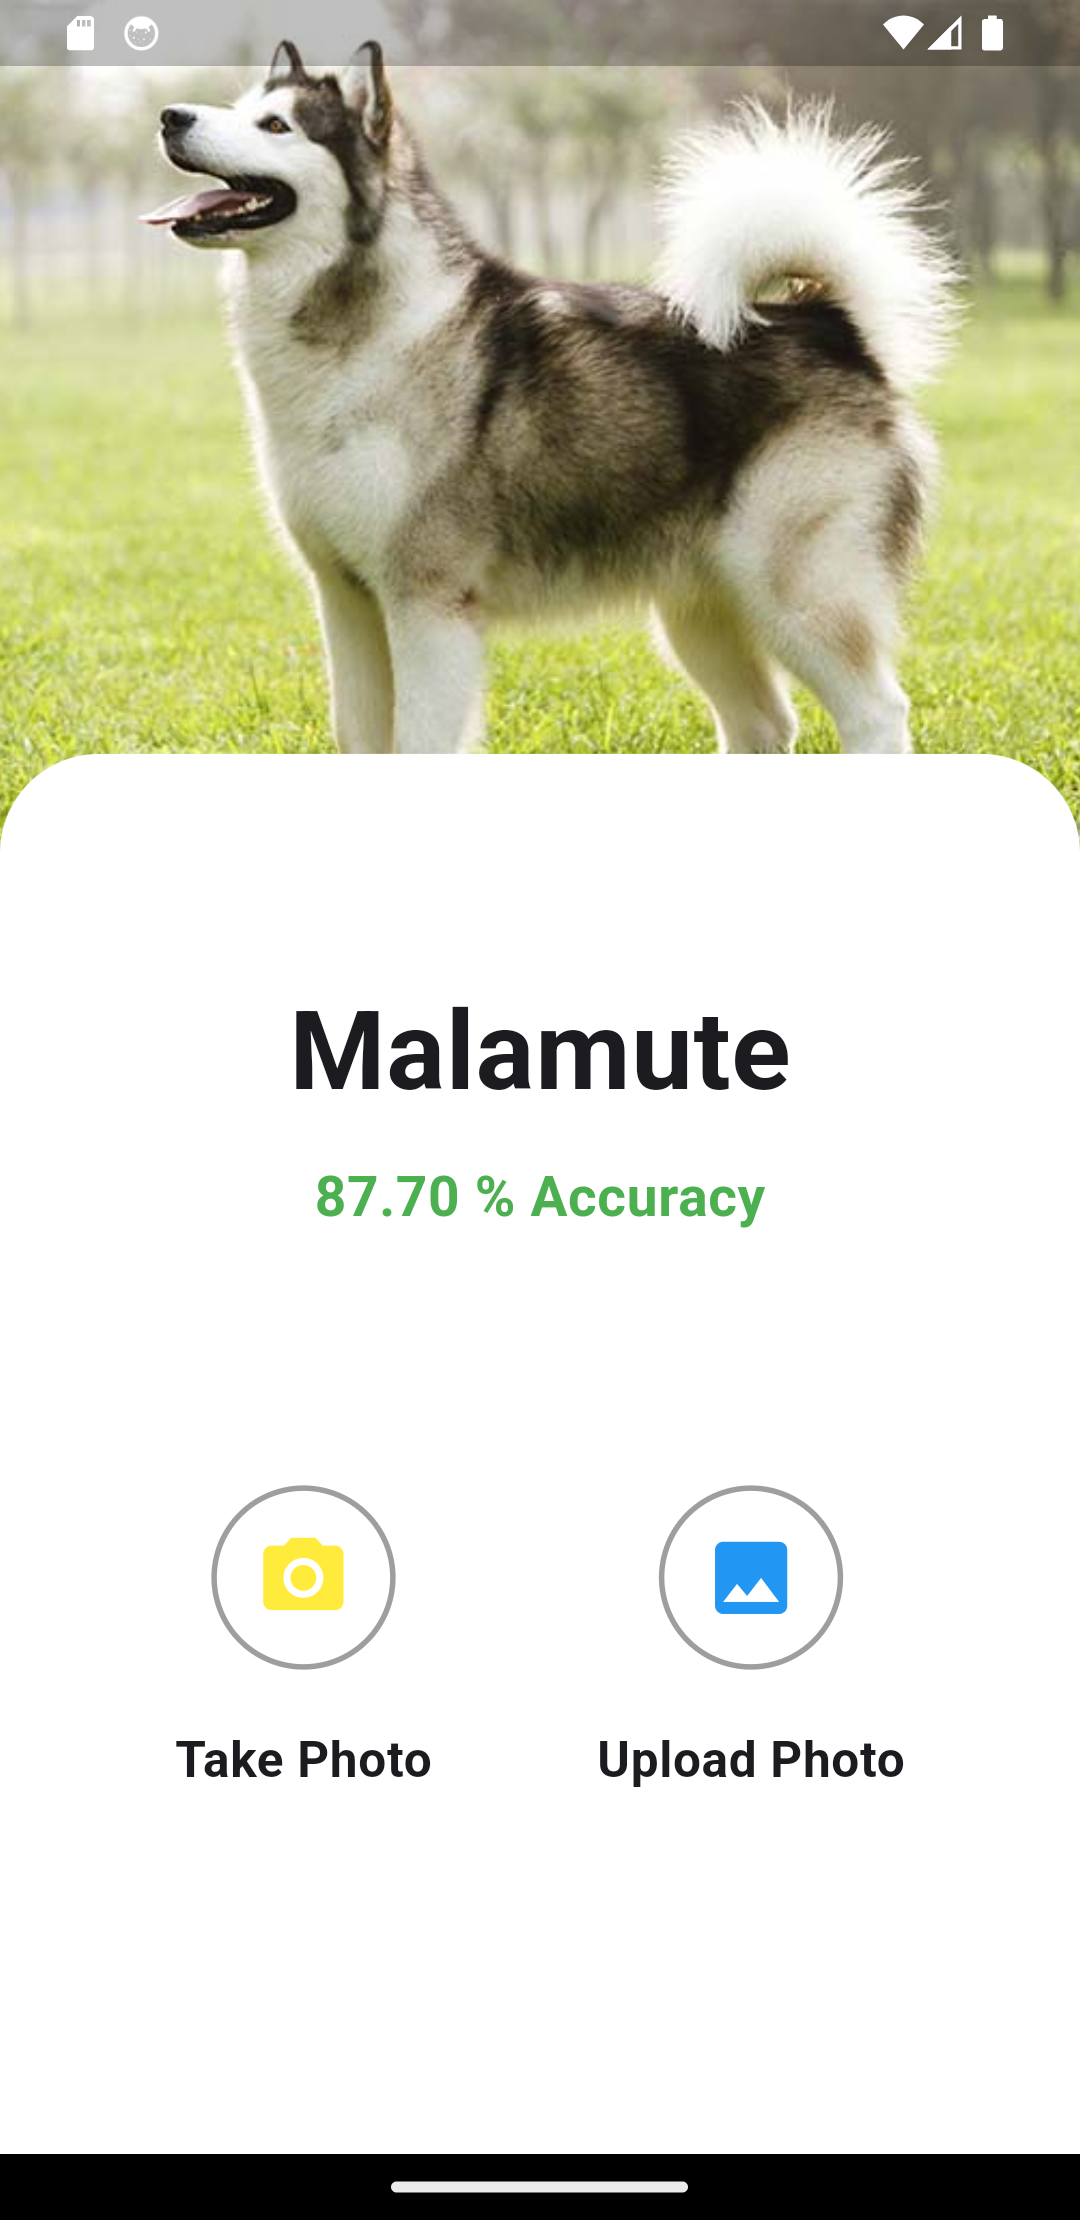
\includegraphics[width=\linewidth]{img/dog5.png}
    % \caption{Subfigure 3}
    \label{subfig:3}
  \end{subfigure}%
  \hfill
  \begin{subfigure}{0.45\textwidth}
    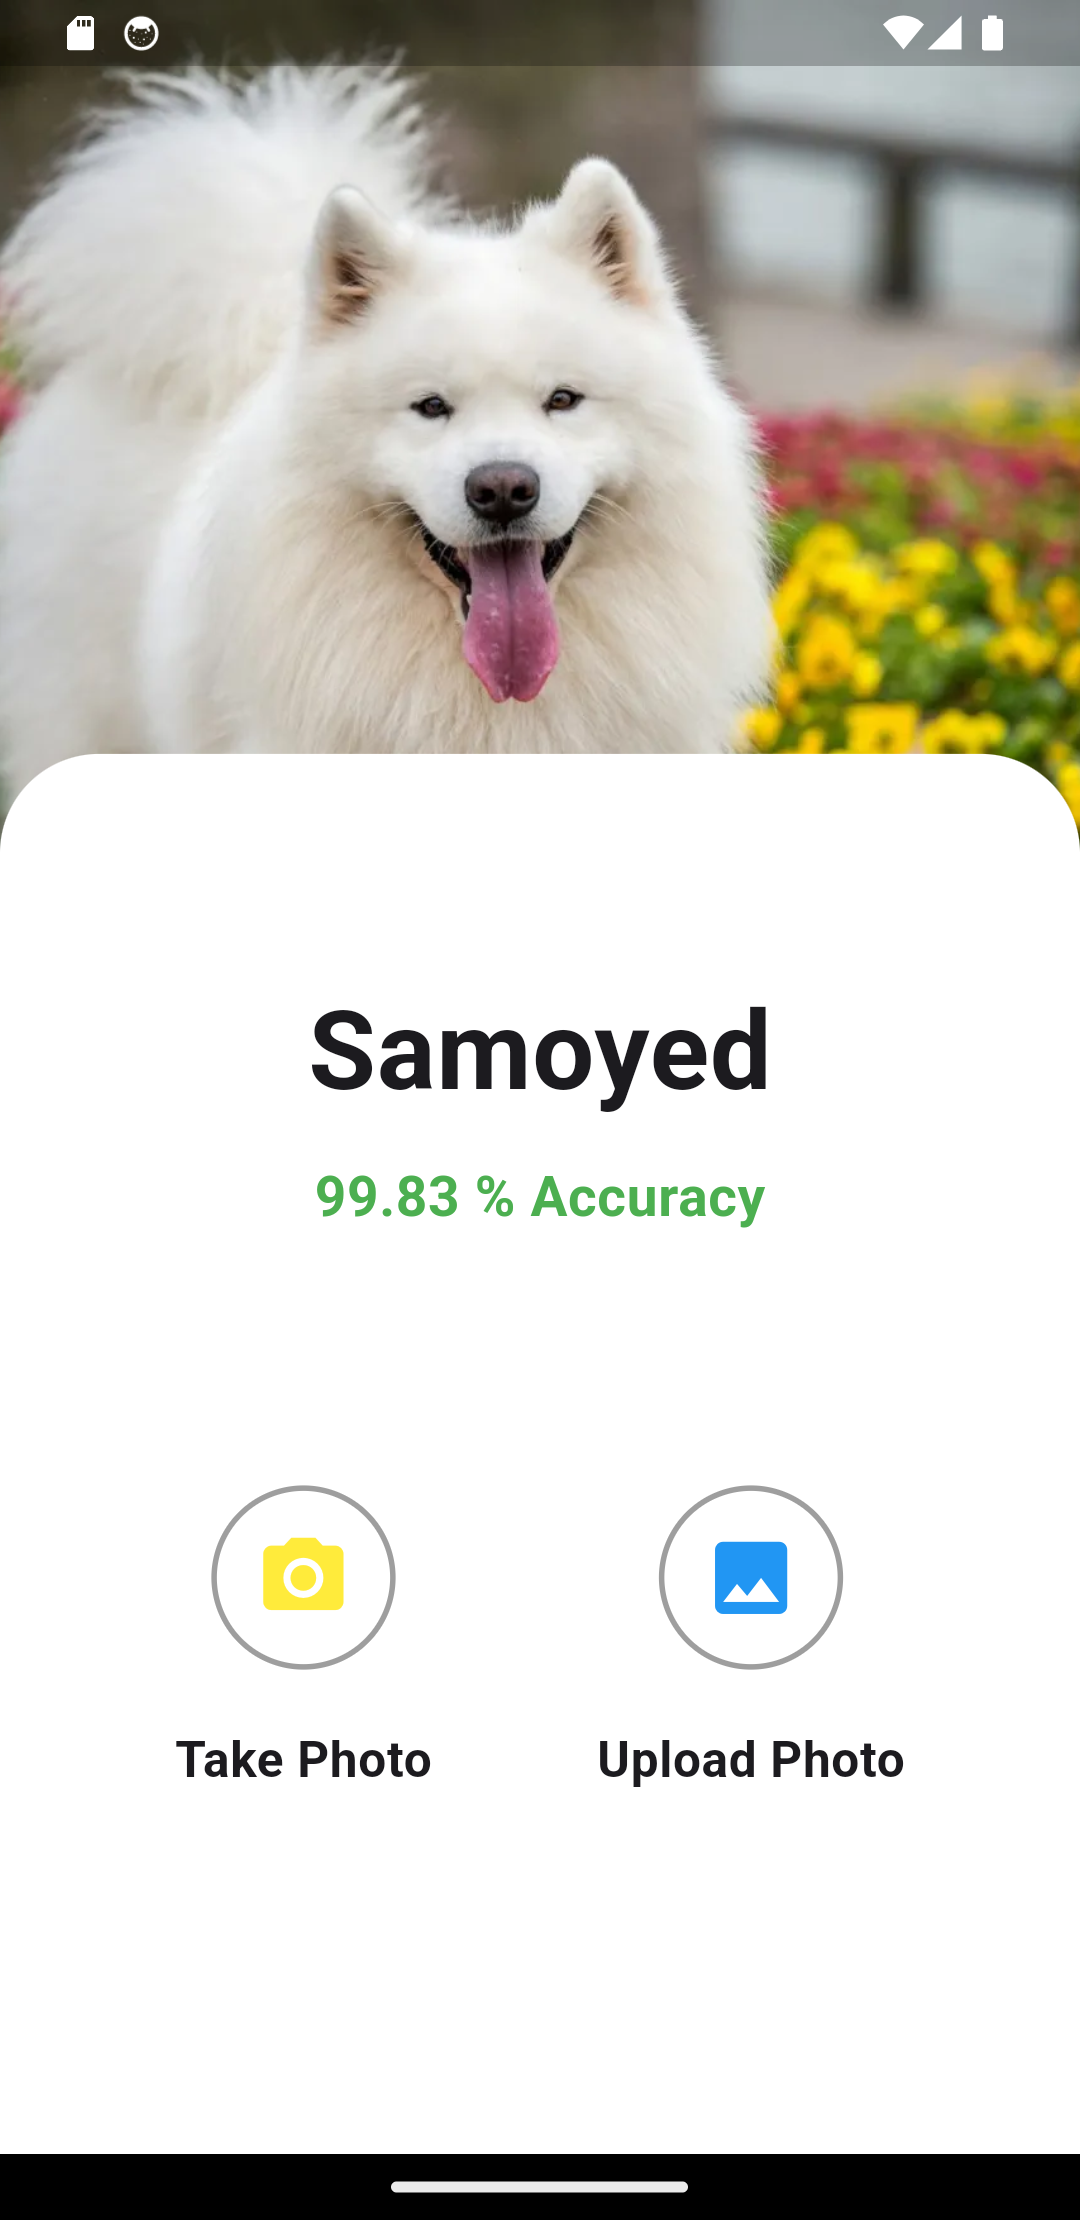
\includegraphics[width=\linewidth]{img/dog7.png}
    % \caption{Subfigure 4}
    \label{subfig:4}
  \end{subfigure}
  \caption{Breed Detection}
  \label{fig:UI Breed Detection}
  \end{figure}
\newpage

\subsubsection{Confusion Matrix}
\vspace{0.7cm}
\begin{figure}[H]
\centering
\includegraphics[width=0.8\linewidth]{img/confusion_matrix.pdf}
\caption{Confusion Matrix}
\label{fig:system-overview}
\end{figure}
The breed detection feature within the HelloPet app has been a pivotal component, elevating the application's functionality for pet owners. In our evaluation, we employed a 120x120 confusion matrix to assess the accuracy of the breed detection algorithm. The matrix served as a comprehensive representation of the diverse pet breeds available, providing insights into the model's performance across various classifications. Upon analysis of the confusion matrix, a visually prominent thick diagonal line emerged, symbolizing instances where the predicted breed aligns with the actual breed. This strong diagonal presence signifies a high level of accuracy in the HelloPet app's breed detection capabilities. The impressive accuracy showcased by this diagonal line assures users that the app excels in correctly identifying a wide array of pet breeds, reinforcing its reliability as a pet-centric application. While the primary focus was on the accuracy represented by the diagonal line, a closer examination of the confusion matrix also revealed outliers outside this central trend. These outliers, though present, were notably sparse, indicating that instances of misclassification were infrequent. The minimal occurrence of outliers underscores the overall reliability of the breed detection feature, assuring users that the HelloPet app consistently provides dependable information about their pets' breeds. In essence, the confusion matrix not only highlights accuracy but also reinforces the robustness and consistency of the breed detection algorithm within the HelloPet app.

Addressing the challenge of distinguishing between visually similar breeds like Siberian Husky and Eskimo Dogs demands a comprehensive strategy. Here are targeted enhancements to our model:

\begin{itemize}
  \item \textbf{Fine-grained Feature Extraction:} Develop advanced algorithms to capture nuanced differences in physical characteristics such as fur texture, muzzle shape, eye size, and body proportions. By leveraging these subtle attributes, the model can discern distinct features crucial for accurate classification.

  \item \textbf{Semantic Segmentation:} Implement techniques to partition images into meaningful segments, enabling focused analysis of breed-specific traits. By dissecting images into regions like head, body, and tail, the model gains deeper insights into key distinguishing features, enhancing its ability to discriminate between similar breeds.

  \item \textbf{Attention Mechanisms:} Integrate attention mechanisms to dynamically prioritize relevant regions within images. By directing attention to informative features while suppressing irrelevant details, the model can effectively distinguish between Siberian husky and Eskimo Dogs based on breed-specific characteristics.

  \item \textbf{Domain-specific Data Augmentation:} Augment training data with synthetic images or variations tailored to each breed's unique attributes. By enriching the dataset with diverse environmental settings, such as snow backgrounds or outdoor scenes, the model learns to generalize better and adapt to real-world scenarios, thereby improving its accuracy in breed classification tasks.
\end{itemize}
These refined strategies aim to enhance the model's capability to discern subtle differences between Siberian Husky and Eskimo Dogs, ultimately bolstering its performance in breed detection tasks.
\vspace{1cm}
\begin{figure}[H]
\centering
\includegraphics[width=0.85\linewidth]{img/confusion_matrix1.pdf}
\caption{Confusion matrix of Siberian Husky and Eskimo Dogs}
\label{fig:system-overview}
\end{figure}

The confusion matrix reveals a significant classification error where instances of the "Eskimo dog" class are frequently misclassified as belonging to the "Siberian husky" class by the object recognition model. This indicates that the model struggles to reliably distinguish between these two visually similar dog breeds. The high value in the corresponding cell of the matrix quantifies this systematic error, highlighting a need to improve the model's ability to differentiate Eskimo dogs from their Siberian husky counterparts. Addressing this issue could involve techniques like fine-tuning on more diverse training data for these classes or incorporating breed-specific features to enhance the model's discrimination capabilities.

\newpage
\subsubsection{Training Loss}
The training and validation loss chart illustrates the progression of the breed detection model in the HelloPet app. Starting at a training loss of 2, the model consistently improves, showing a steady decline in error up to epoch 15. The validation loss, slightly higher initially, follows a similar pattern, signifying effective learning but highlighting the model's need for enhanced generalization to unseen data. The persistent gap between training and validation losses suggests a balanced learning process, necessitating ongoing optimization to maximize performance on diverse pet breeds.
\vspace{1cm}
\begin{figure}[H]
\centering
\includegraphics[width=0.85\linewidth]{img/valid 1.pdf}
\caption{Training loss}
\label{fig:system-overview}
\end{figure}

\newpage

\subsubsection{Accuracy}
Below is the graph depicting accuracy over each epoch. Notably, the accuracy exhibited a sharp increase from the first to the second epoch, followed by a gradual rise over subsequent epochs, culminating in a final accuracy of 95.47\% after 15 epochs.
\vspace{1cm}
\begin{figure}[H]
\centering
\vspace{0.7cm}
\begin{figure}[H]
\centering
\includegraphics[width=1\linewidth]{img/valid 2.pdf}
\caption{Accuracy curve}
\label{fig:system-overview}
\end{figure}
\newpage
\label{fig:system-overview}
\end{figure}
\newpage
\subsection{Community}
The community feature encompasses diverse elements such as user profiles, pages, and posts, requiring database establishment and backend development, both of which have been successfully implemented. Additionally, the UI development for these features has been completed, ensuring a comprehensive and seamless user experience. The community section's UI enhancements have been finalized, marking the successful conclusion of the overall UI development process.

\vspace{1cm}
\begin{figure}[ht]
  \centering
    \begin{subfigure}{0.3\textwidth}
    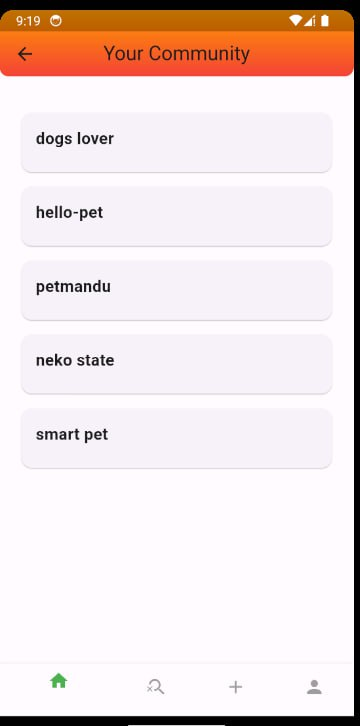
\includegraphics[width=\linewidth]{img/community.jpg}
  \end{subfigure}%
  \hfill
  \begin{subfigure}{0.31\textwidth}
    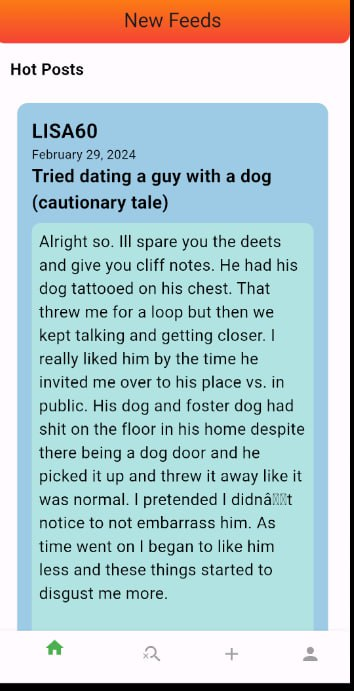
\includegraphics[width=\linewidth]{img/hot feed.jpg}
  \end{subfigure}%
  \hfill
  \begin{subfigure}{0.3\textwidth}
    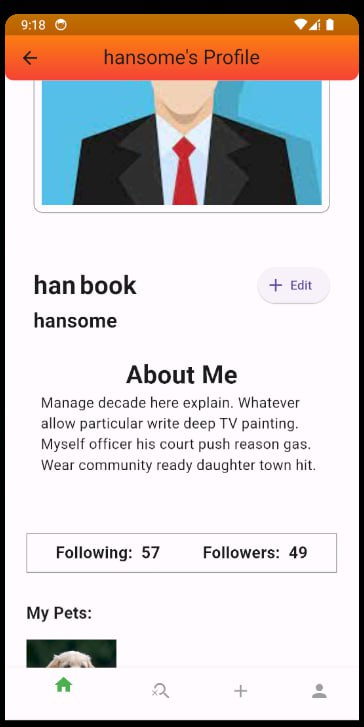
\includegraphics[width=\linewidth]{img/profile.jpg}
  \end{subfigure}%
 \caption{Community}
  \label{fig:UI}
\end{figure}